\chapter{Brought into Glory by Grace (21:1--22:21)}\index{glory}\index{grace}

At last, we have arrived at the new heaven and the new earth. Someone might ask, ``I have not even finished my journey through this life. Why should I already be longing for the new heaven and the new earth of eternity?''

Let me offer a simple illustration.

Imagine that you are preparing to move into a spacious, beautiful new home. Everything has been made ready, and you know that one day you will live there. Yet the children and teenagers in your household are reluctant to leave the house. They might say, ``Isn't it good enough to live here? Why do we have to move?'' Would you respond to them that, if they feel that way, you will simply abandon the move? Of course not. Instead, you would take them to see the new home. You would help them imagine the life that awaits them. 

Hebrews 11:16 reminds us that God's people are strangers and pilgrims on the earth, longing for a better place, a heavenly one. God has prepared a city for them. And when the Lord Jesus was preparing to depart from His disciples, He told them that He was going to prepare a place for them (John 14:2). Our hope in the new heaven and the new earth rests on this same promise.

We do not long for the life to come because we despise the life we have now. We come to know Christ, learn to love others, and serve our Lord. Yet we know that even these precious gifts are not the end of the story.

God has prepared a better place for His people: a glorious\index{glory} dwelling in which He will renew heaven and earth and live among them forever.

Therefore, Christians can cherish the present while looking forward to that day. We can faithfully complete the journey set before us while lifting our eyes toward the glory that lies ahead.

\begin{figure}[h]
    \centering
    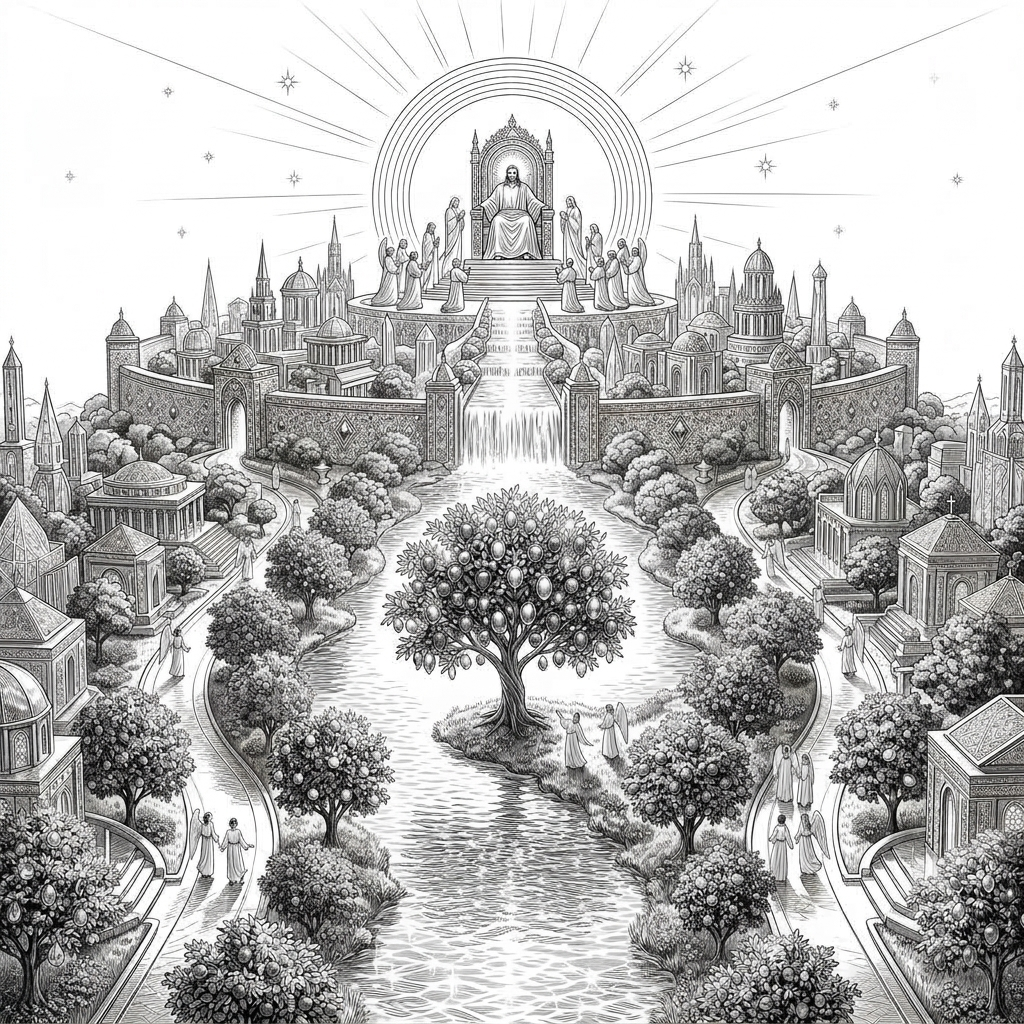
\includegraphics[
    width=1\textwidth,
    trim=0 0 0 0,
    clip]{images/tree_of_life.jpg}
\end{figure}

\section{All Things Made New: God Dwelling with His People}

\begin{ScriptureBox}

\item[21:1] Then I saw ``a new heaven and a new earth,'' for the first heaven and the first earth had passed away, and there was no longer any sea.
% NIV footnote for 21:1: ``a new heaven and a new earth'' --- Isaiah 65:17

\item[21:2] I saw the Holy City, the new Jerusalem, coming down out of heaven from God, prepared as a bride beautifully dressed for her husband.

\item[21:3] And I heard a loud voice from the throne saying, ``Look! God's dwelling place is now among the people, and he will dwell with them. They will be his people, and God himself will be with them and be their God.

\item[21:4] `He will wipe every tear from their eyes. There will be no more death' or mourning or crying or pain, for the old order of things has passed away.''
% NIV footnote for 21:4: ``no more death'' --- Isaiah 25:8
% CHECK NIV: footnote references for 21:1 and 21:4 quoted from memory;
%   verify against Bible Gateway.

\item[21:5] He who was seated on the throne said, ``I am making everything new!'' Then he said, ``Write this down, for these words are trustworthy and true.''

\item[21:6] He said to me: ``It is done. I am the Alpha and the Omega, the Beginning and the End. To the thirsty I will give water without cost from the spring of the water of life.

\item[21:7] Those who are victorious will inherit all this, and I will be their God and they will be my children.

\item[21:8] But the cowardly, the unbelieving, the vile, the murderers, the sexually immoral, those who practice magic arts, the idolaters and all liars---they will be consigned to the fiery lake of burning sulfur. This is the second death.''

\end{ScriptureBox}

One word stands out as we read about the new heaven and the new earth and the New Jerusalem\index{New Jerusalem}: \textbf{new}. But what does this newness mean?

If we were to enter the new heaven and the new earth still as the people we once were, with our old lives, our old dispositions, and our old sins, would we not be out of place in such a holy dwelling? God is not merely renewing the heavens and the earth. He is also renewing His people, preparing them to live with Him forever.

Paul writes that although our outward nature is wasting away, our inward nature is being renewed day by day (2 Corinthians 4:16). Our renewal does not begin only when we enter the new heaven and the new earth. It has already begun in Christ. Today, God is at work transforming us; on that day, He will bring His work to completion.

Consider the robber who was crucified beside Jesus. He had lived a sinful life and was dying under the sentence of his own wrongdoing. Yet, in his final hours, he recognized something extraordinary in the Man who hung beside him. He acknowledged his own guilt and asked Jesus to remember him.

Jesus answered him with the promise of paradise (Luke 23:43).

The man had no time to rebuild his life, no opportunity to establish a record of good works or prove through years of conduct that he had changed. Yet his heart turned toward Christ. The man who had lived in sin now looked to Jesus and entrusted himself to Him.

This is the transforming power of grace\index{grace}.

The new heaven and the new earth will not be inhabited by people who remain devoted to sin. They will be God's redeemed\index{redemption} people, whom He has already begun to renew in Christ, whom He continues to transform in this life, and whom He will one day glorify completely.

Who is the One who makes all things new?

He declares, ``It is done.'' He is the Alpha and the Omega\index{Alpha and Omega}, the Beginning and the End. He freely gives the water of life\index{water of life} to the thirsty.

We are reminded of Jesus' encounter with the Samaritan woman at Jacob's well. There, He promised that whoever drinks the water He gives will never thirst again, for His gift becomes a spring welling up to eternal life (John 4:14).

The One who promises to renew all things is the same One who offers us living water today. The life of the coming age is not a distant hope detached from our present walk with Him. 

\section{The Bride Is the New Jerusalem}\index{New Jerusalem}\index{bride of the Lamb}

\begin{ScriptureBox}

\item[21:9] One of the seven angels who had the seven bowls full of the seven last plagues came and said to me, ``Come, I will show you the bride, the wife of the Lamb.''

\item[21:10] And he carried me away in the Spirit to a mountain great and high, and showed me the Holy City, Jerusalem, coming down out of heaven from God.

\item[21:11] It shone with the glory of God, and its brilliance was like that of a very precious jewel, like a jasper, clear as crystal.

\item[21:12] It had a great, high wall with twelve gates, and with twelve angels at the gates. On the gates were written the names of the twelve tribes of Israel.

\item[21:13] There were three gates on the east, three on the north, three on the south and three on the west.

\item[21:14] The wall of the city had twelve foundations, and on them were the names of the twelve apostles of the Lamb.

\item[21:15] The angel who talked with me had a measuring rod of gold to measure the city, its gates and its walls.

\item[21:16] The city was laid out like a square, as long as it was wide. He measured the city with the rod and found it to be 12,000 stadia in length, and as wide and high as it is long.
% NIV footnote for 21:16: ``12,000 stadia'' --- That is, about 1,400 miles
%   or about 2,200 kilometers

\item[21:17] The angel measured the wall using human measurement, and it was 144 cubits thick.
% NIV footnotes for 21:17:
%   ``144 cubits'' --- That is, about 200 feet or about 65 meters
%   ``thick'' --- Or high

\item[21:18] The wall was made of jasper, and the city of pure gold, as pure as glass.

\item[21:19] The foundations of the city walls were decorated with every kind of precious stone. The first foundation was jasper, the second sapphire, the third agate, the fourth emerald,

\item[21:20] the fifth onyx, the sixth ruby, the seventh chrysolite, the eighth beryl, the ninth topaz, the tenth turquoise, the eleventh jacinth, and the twelfth amethyst.
% NIV footnote for 21:20: end of verse --- The precise identification of
%   some of these precious stones is uncertain.
% CHECK NIV: footnote wording for 21:16--20 quoted from memory;
%   verify against Bible Gateway.

\item[21:21] The twelve gates were twelve pearls, each gate made of a single pearl. The great street of the city was of gold, as pure as transparent glass.

\end{ScriptureBox}

The holy city\index{holy city} descends from heaven, radiant with splendor and filled with the glory of God. John looks upon it carefully, taking in its gates, its foundations, and its extraordinary beauty.

There are three gates on each side of the city, and the names of the twelve tribes\index{twelve tribes of Israel} of Israel\index{Israel} are written upon them. The city wall rests on twelve foundations, bearing the names of the Lamb\index{Lamb, the}'s twelve apostles.

This vision calls to mind Jesus' words to Peter: He would build His church upon the rock, and the gates of Hades\index{Hades} would not overcome\index{overcomers} it (Matthew 16:18).

The New Jerusalem\index{New Jerusalem} has twelve foundations associated with the twelve apostles of the New Testament and twelve gates bearing the names of the twelve tribes\index{twelve tribes of Israel} of Israel. Together, these features point to the unity and completeness of God's redemptive purpose. The people of God in the Old Testament and the redeemed community gathered through Christ are brought together in one glorious dwelling.

This does not erase the distinction between Israel and the Church in every theological discussion. Rather, the imagery shows that God's saving purpose reaches its fulfillment in the city He has prepared for His people, a city whose foundations and gates bear witness to the unfolding story of redemption.

For Christians, this vision also affirms that our faith is firmly grounded. As Ephesians 2:20 teaches, God's household is built on the foundation of the apostles and prophets, with Christ Jesus Himself as the chief cornerstone.

The city is given precise measurements, suggesting perfection, holiness, and completeness. It is shaped like a perfect cube, with its length, width, and height equal. Its dimensions are twelve thousand \textit{stadia.}
In modern measurements, twelve thousand stadia is approximately 1,400 miles, or about 2,250 kilometers.

Imagine, then, a city whose length, width, and height each extend for roughly 1,400 miles. Picture an immense cube, radiant with the glory of God, rising far beyond the scale of anything we have known.

\begin{figure}[htbp]
    \centering
    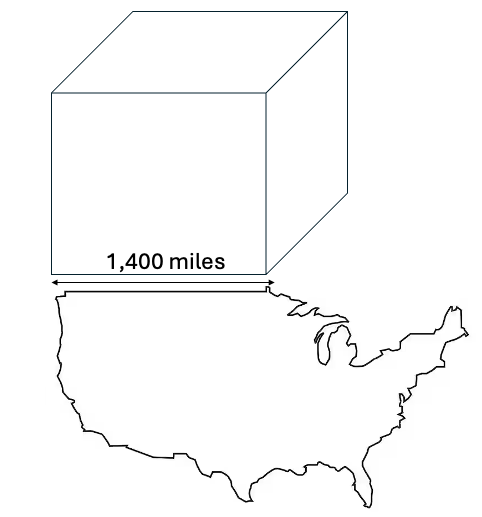
\includegraphics[
    width=0.6\textwidth,
    trim=0 0 0 0,
    clip]{images/new_jesusalem_US.png}
\end{figure}


What a magnificent city!

And Revelation 7:9 has already shown us an innumerable multitude standing before the throne\index{throne of God} and before the Lamb, drawn from every nation, tribe, people, and language.

The vision invites us to imagine the vastness of the redeemed community dwelling in God's presence, no longer divided by hostility or separated from Him by sin and death. The dimensions of the city are not given to satisfy our curiosity alone. They direct our attention toward the greatness of the God who prepares such a dwelling for His people.

This comparison is only a small aid to our imagination. The glory of the New Jerusalem\index{New Jerusalem} exceeds anything we can fully comprehend. As Paul reminds us, God has prepared things for those who love Him that human eyes have not seen, ears have not heard, and hearts have not conceived (1 Corinthians 2:9).


\section{God Himself Is the Temple of the City}\index{temple}

\begin{ScriptureBox}

\item[21:22] I did not see a temple in the city, because the Lord God Almighty and the Lamb are its temple.

\item[21:23] The city does not need the sun or the moon to shine on it, for the glory of God gives it light, and the Lamb is its lamp.

\item[21:24] The nations will walk by its light, and the kings of the earth will bring their splendor into it.

\item[21:25] On no day will its gates ever be shut, for there will be no night there.

\item[21:26] The glory and honor of the nations will be brought into it.

\item[21:27] Nothing impure will ever enter it, nor will anyone who does what is shameful or deceitful, but only those whose names are written in the Lamb's book of life.

\end{ScriptureBox}

Those who dwell in the city are people who have been saved by grace. Their names are written in the Lamb's book of life\index{book of life}. They are the work of God's grace.

In Christ, God has chosen, called, forgiven, and preserved His people, bringing them at last into the eternal city He has prepared. Their presence there is not the reward of human achievement, but the fulfillment of God's saving purpose.

The redeemed share a common identity: they belong to the Lamb who gave Himself for them. Yet the vision also preserves the richness of the nations. The glory of the city is not portrayed as the erasure of every distinction among peoples. Rather, the nations bring their splendor into the light of God's presence.

Differences that once became occasions for division no longer stand in opposition to the worship\index{worship} of God. The redeemed gather in unity, and the diversity of the nations becomes part of the rich beauty of their common praise.

What a beautiful vision of the people of God, gathered at last in the light of His glory!

And at the heart of it all stands a remarkable truth: there is no temple\index{temple} in the city. God's people no longer approach Him through an earthly sanctuary, for the Lord God Almighty and the Lamb are themselves the temple. The presence for which the people of God have longed throughout the ages is now their everlasting home.

\begin{ReaderQuestion}
From the Garden of Eden, through the tabernacle and the temple, to the incarnation of Christ and finally the new heaven and the new earth, how do you see God's promise to dwell with His people unfolding throughout the Bible?
\end{ReaderQuestion}

\section{The River of Life and the Tree of Life}\index{water of life}\index{tree of life}

\begin{ScriptureBox}

\item[22:1] Then the angel showed me the river of the water of life, as clear as crystal, flowing from the throne of God and of the Lamb

\item[22:2] down the middle of the great street of the city. On each side of the river stood the tree of life, bearing twelve crops of fruit, yielding its fruit every month. And the leaves of the tree are for the healing of the nations.

\item[22:3] No longer will there be any curse. The throne of God and of the Lamb will be in the city, and his servants will serve him.

\item[22:4] They will see his face, and his name will be on their foreheads.

\item[22:5] There will be no more night. They will not need the light of a lamp or the light of the sun, for the Lord God will give them light. And they will reign for ever and ever.

\end{ScriptureBox}

The opening verses of Revelation 22 bring us back to the Garden of Eden\index{Eden} in Genesis. There, we encountered the tree of life\index{tree of life} and the river that watered the garden. Here, the river of the water of life\index{water of life} flows from the throne of God and of the Lamb.

Human life depends upon God and finds its fullest joy in Him. Life is His gift, and the blessings of the new creation flow from His presence. The tree of life\index{tree of life} bears fruit every month, continually sustaining the life and flourishing of God's people.

John also tells us that the leaves of the tree are for the healing of the nations. This does not necessarily imply that disease will persist in the new creation. In the context of a world where death, pain, and the curse have been abolished, the imagery points toward the complete restoration and enduring well-being of the nations. The tree represents the fullness of life God provides, not a continuing struggle against illness.\footnote{See John MacArthur's discussion of Revelation 22 in his commentary on Revelation (2007).}

Verse 3 declares that there will no longer be any curse. These words take us back to Genesis 3, where sin entered the world and the curse followed. Now, in Revelation 22, redemption has reached its fulfillment, and the curse is removed forever.

Table \ref{tab:genesis3-rev21-22} shows the comparison between the beginning and the end of the biblical story.

{
\renewcommand{\arraystretch}{1}
\small
\begin{longtable}{>{\raggedright\arraybackslash}p{0.45\textwidth} >{\raggedright\arraybackslash}p{0.45\textwidth}}
\caption{Paradise lost and paradise restored: Genesis 3 and Revelation 21--22}
\label{tab:genesis3-rev21-22} \\
\hline
\textbf{Genesis 3} & \textbf{Revelation 21--22} \\
\hline
\endfirsthead

\multicolumn{2}{l}{\small\itshape Table~\thetable\ (continued)} \\
\hline
\textbf{Genesis 3} & \textbf{Revelation 21--22} \\
\hline
\endhead

\hline
\endfoot

\hline
\endlastfoot

Sin enters the world & All things are made new \\
The curse falls upon creation & There is no more curse \\
Humanity is driven from Eden & God's people enter the holy city \\
Access to the tree of life is lost & God's people receive the blessings of the tree of life \\
Humanity is separated from God & God dwells with His people \\
Death enters the world & Death is no more \\
The serpent deceives humanity & Satan is utterly defeated \\
Humanity loses the joy of God's presence & God's servants see His face \\
\end{longtable}
}


The Bible's story begins in a garden and reaches its fulfillment in a city. What was lost through sin is restored through the saving work of God. Yet the final vision is more than a return to Eden\index{Eden}. The redeemed dwell in the presence of God and the Lamb, their fellowship with Him no longer threatened by sin, suffering, or death.

The story that began with the tragedy of human rebellion ends with the triumph of divine grace.

\section{Do Not Seal Up the Words of This Book}

Now the book of Revelation speaks directly to us. The angel declares that these words are trustworthy and true. 

\begin{ScriptureBox}

\item[22:6] The angel said to me, ``These words are trustworthy and true. The Lord, the God who inspires the prophets, sent his angel to show his servants the things that must soon take place.''

\item[22:7] ``Look, I am coming soon! Blessed is the one who keeps the words of the prophecy written in this scroll.''

\item[22:8] I, John, am the one who heard and saw these things. And when I had heard and seen them, I fell down to worship at the feet of the angel who had been showing them to me.

\item[22:9] But he said to me, ``Don't do that! I am a fellow servant with you and with your fellow prophets and with all who keep the words of this scroll. Worship God!''

\item[22:10] Then he told me, ``Do not seal up the words of the prophecy of this scroll, because the time is near.

\item[22:11] Let the one who does wrong continue to do wrong; let the vile person continue to be vile; let the one who does right continue to do right; and let the holy person continue to be holy.''

\item[22:12] ``Look, I am coming soon! My reward is with me, and I will give to each person according to what they have done.

\item[22:13] I am the Alpha and the Omega, the First and the Last, the Beginning and the End.

\item[22:14] ``Blessed are those who wash their robes, that they may have the right to the tree of life and may go through the gates into the city.

\item[22:15] Outside are the dogs, those who practice magic arts, the sexually immoral, the murderers, the idolaters and everyone who loves and practices falsehood.

\end{ScriptureBox}

They were not given merely to satisfy curiosity about the future. They were given to God's people to be read, heard, kept, and obeyed.


Once again, we hear Jesus declare who He is:

``I am the Alpha and the Omega\index{Alpha and Omega}, the First and the Last, the Beginning and the End.''

Alpha is the first letter of the Greek alphabet, and Omega is the last. The whole course of history lies under His sovereign rule. From creation to the new heaven and the new earth, from the cross to glory, nothing lies beyond His authority or outside His redemptive purpose.

We also encounter a solemn statement: the one who does wrong will continue to do wrong, and the one who is holy will continue to be holy. These words should not be taken as permission to remain in sin. Rather, they confront us with the seriousness of the paths we choose and the loyalties we cultivate.

As history approaches its appointed end, the true character of human lives will be revealed. The fruit of a person's life will bear witness to the direction of the heart and to the allegiance that has shaped it. The final judgment\index{judgment} will expose what has been hidden, and no outward appearance will conceal the truth.

This warning calls us to examine ourselves before God. It also reminds us that the present is a time of grace, a time to turn from sin, trust in Christ, and walk in the holiness He gives His people.

The One who is coming is also the One who sees us now. His promise is certain, His judgment is righteous, and His invitation remains open.

\section{The Final Gospel Invitation: Let the Thirsty Come}

\begin{ScriptureBox}

\item[22:16] ``I, Jesus, have sent my angel to give you this testimony for the churches. I am the Root and the Offspring of David, and the bright Morning Star.''
% NIV footnote for 22:16 (omitted; add as \footnote if wanted):
%   ``you'' --- The Greek is plural.
% CHECK NIV: footnote wording quoted from memory; verify against Bible Gateway.

\item[22:17] The Spirit and the bride say, ``Come!'' And let the one who hears say, ``Come!'' Let the one who is thirsty come; and let the one who wishes take the free gift of the water of life.

\end{ScriptureBox}

At the end of Revelation, we hear one final invitation, addressed to everyone who reads these words and still thirsts for life:

``Let the thirsty come; and let the one who wishes take the free gift of the water of life\index{water of life}'' (Revelation 22:17, NIV).

What a beautiful gospel invitation!

It brings us back to Jesus' conversation with the Samaritan woman at the well. He promised that whoever drinks the water He gives will never thirst again, for that water becomes a spring welling up to eternal life (John 4:14).

The invitation is not a call to earn eternal life through human achievement. It is an invitation to receive what God freely gives. The thirsty are not told to make themselves worthy before approaching Him. They are invited to come.

God's purpose is to bring people into the glory of eternal life, where they will drink deeply of the life He provides and dwell in His presence forever.

The gospel invitation also reveals the heart of the One who calls us. The God who will judge the world is the same God who offers the water of life\index{water of life} freely. The Lamb who will bring history to its appointed end is the Lamb who gave His life to redeem His people.

The final invitation of Scripture therefore remains open to all who will come to Christ in faith. The thirsty may come. The weary may come. Those who know their need may come. The gift is not purchased by merit; it is received through grace.

\begin{ReaderQuestion}
If you were explaining Revelation 22:17 to someone who does not yet believe in Christ but feels a deep thirst in life, how would you describe the invitation? How does this verse show that the gospel is a gift of grace rather than something we purchase through good deeds or personal merit?
\end{ReaderQuestion}

\section{``Come, Lord Jesus''}

\begin{ScriptureBox}

\item[22:18] I warn everyone who hears the words of the prophecy of this scroll: If anyone adds anything to them, God will add to that person the plagues described in this scroll.

\item[22:19] And if anyone takes words away from this scroll of prophecy, God will take away from that person any share in the tree of life and in the Holy City, which are described in this scroll.

\item[22:20] He who testifies to these things says, ``Yes, I am coming soon.''\\
Amen. Come, Lord Jesus.

\item[22:21] The grace of the Lord Jesus be with God's people. Amen.

\end{ScriptureBox}

Revelation closes with two voices answering one another. The Lord Jesus declares, ``I am coming soon,'' and the Church responds, ``Amen. Come, Lord Jesus.''

Their exchange reminds us of the longing expressed in the Song of Songs, where the beloved longs for the arrival of the one she loves. The bride\index{bride of the Lamb}'s deepest desire is not merely to enjoy a wedding feast, but to be with her beloved.

So it is with the Church. Our hope is not simply that suffering will end, that injustice will be put right, or that the world will finally be made whole. These promises are precious, but at the heart of our hope stands a Person: Jesus Christ, the Lamb who loved us, gave Himself for us, and rose from the dead.

We long for Him to come.

His promise, ``I am coming soon,'' sustains us as we wait. It gives us courage in suffering, steadiness in uncertainty, and strength to remain faithful when the road grows difficult. We do not know every detail of the journey ahead, but we know the One who holds its end in His hands.

The final words of Revelation are therefore not merely a prediction about the future. They are the confession of a people whose hearts have been captured by grace. We have been called by Christ, redeemed by His blood, renewed by His Spirit, and promised a place in the city where God will dwell with His people forever.

And so we wait—not with empty hands or hopeless hearts, but with our eyes fixed on the returning King.

``Amen. Come, Lord Jesus.''

\begin{ReaderQuestion}
What does ``Come, Lord Jesus'' mean to you? How can this longing become more than a hope for the future and shape your prayers and choices today? In your work, family, suffering, service, and uncertainty about the future, how might the promise of Christ's return change the way you live?
\end{ReaderQuestion}
